\begin{frame}
\frametitle{Pilot Logbooks}
\begin{block}{CASR1998 REG 61.345 \emph{(pilot logbooks)}}
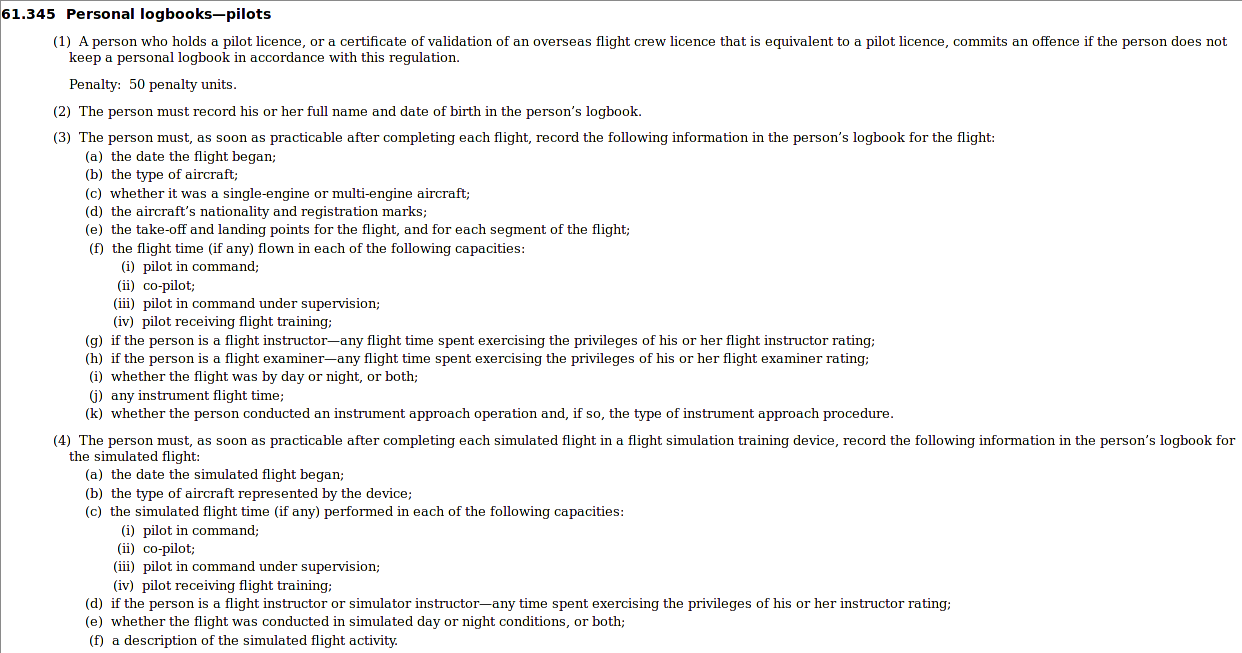
\includegraphics[height=0.6\textheight]{image/casr-logbook.png}
\end{block}
\end{frame}

\begin{frame}
\frametitle{Pilot Logbooks}
\begin{block}{Here is a typical pilot logbook}
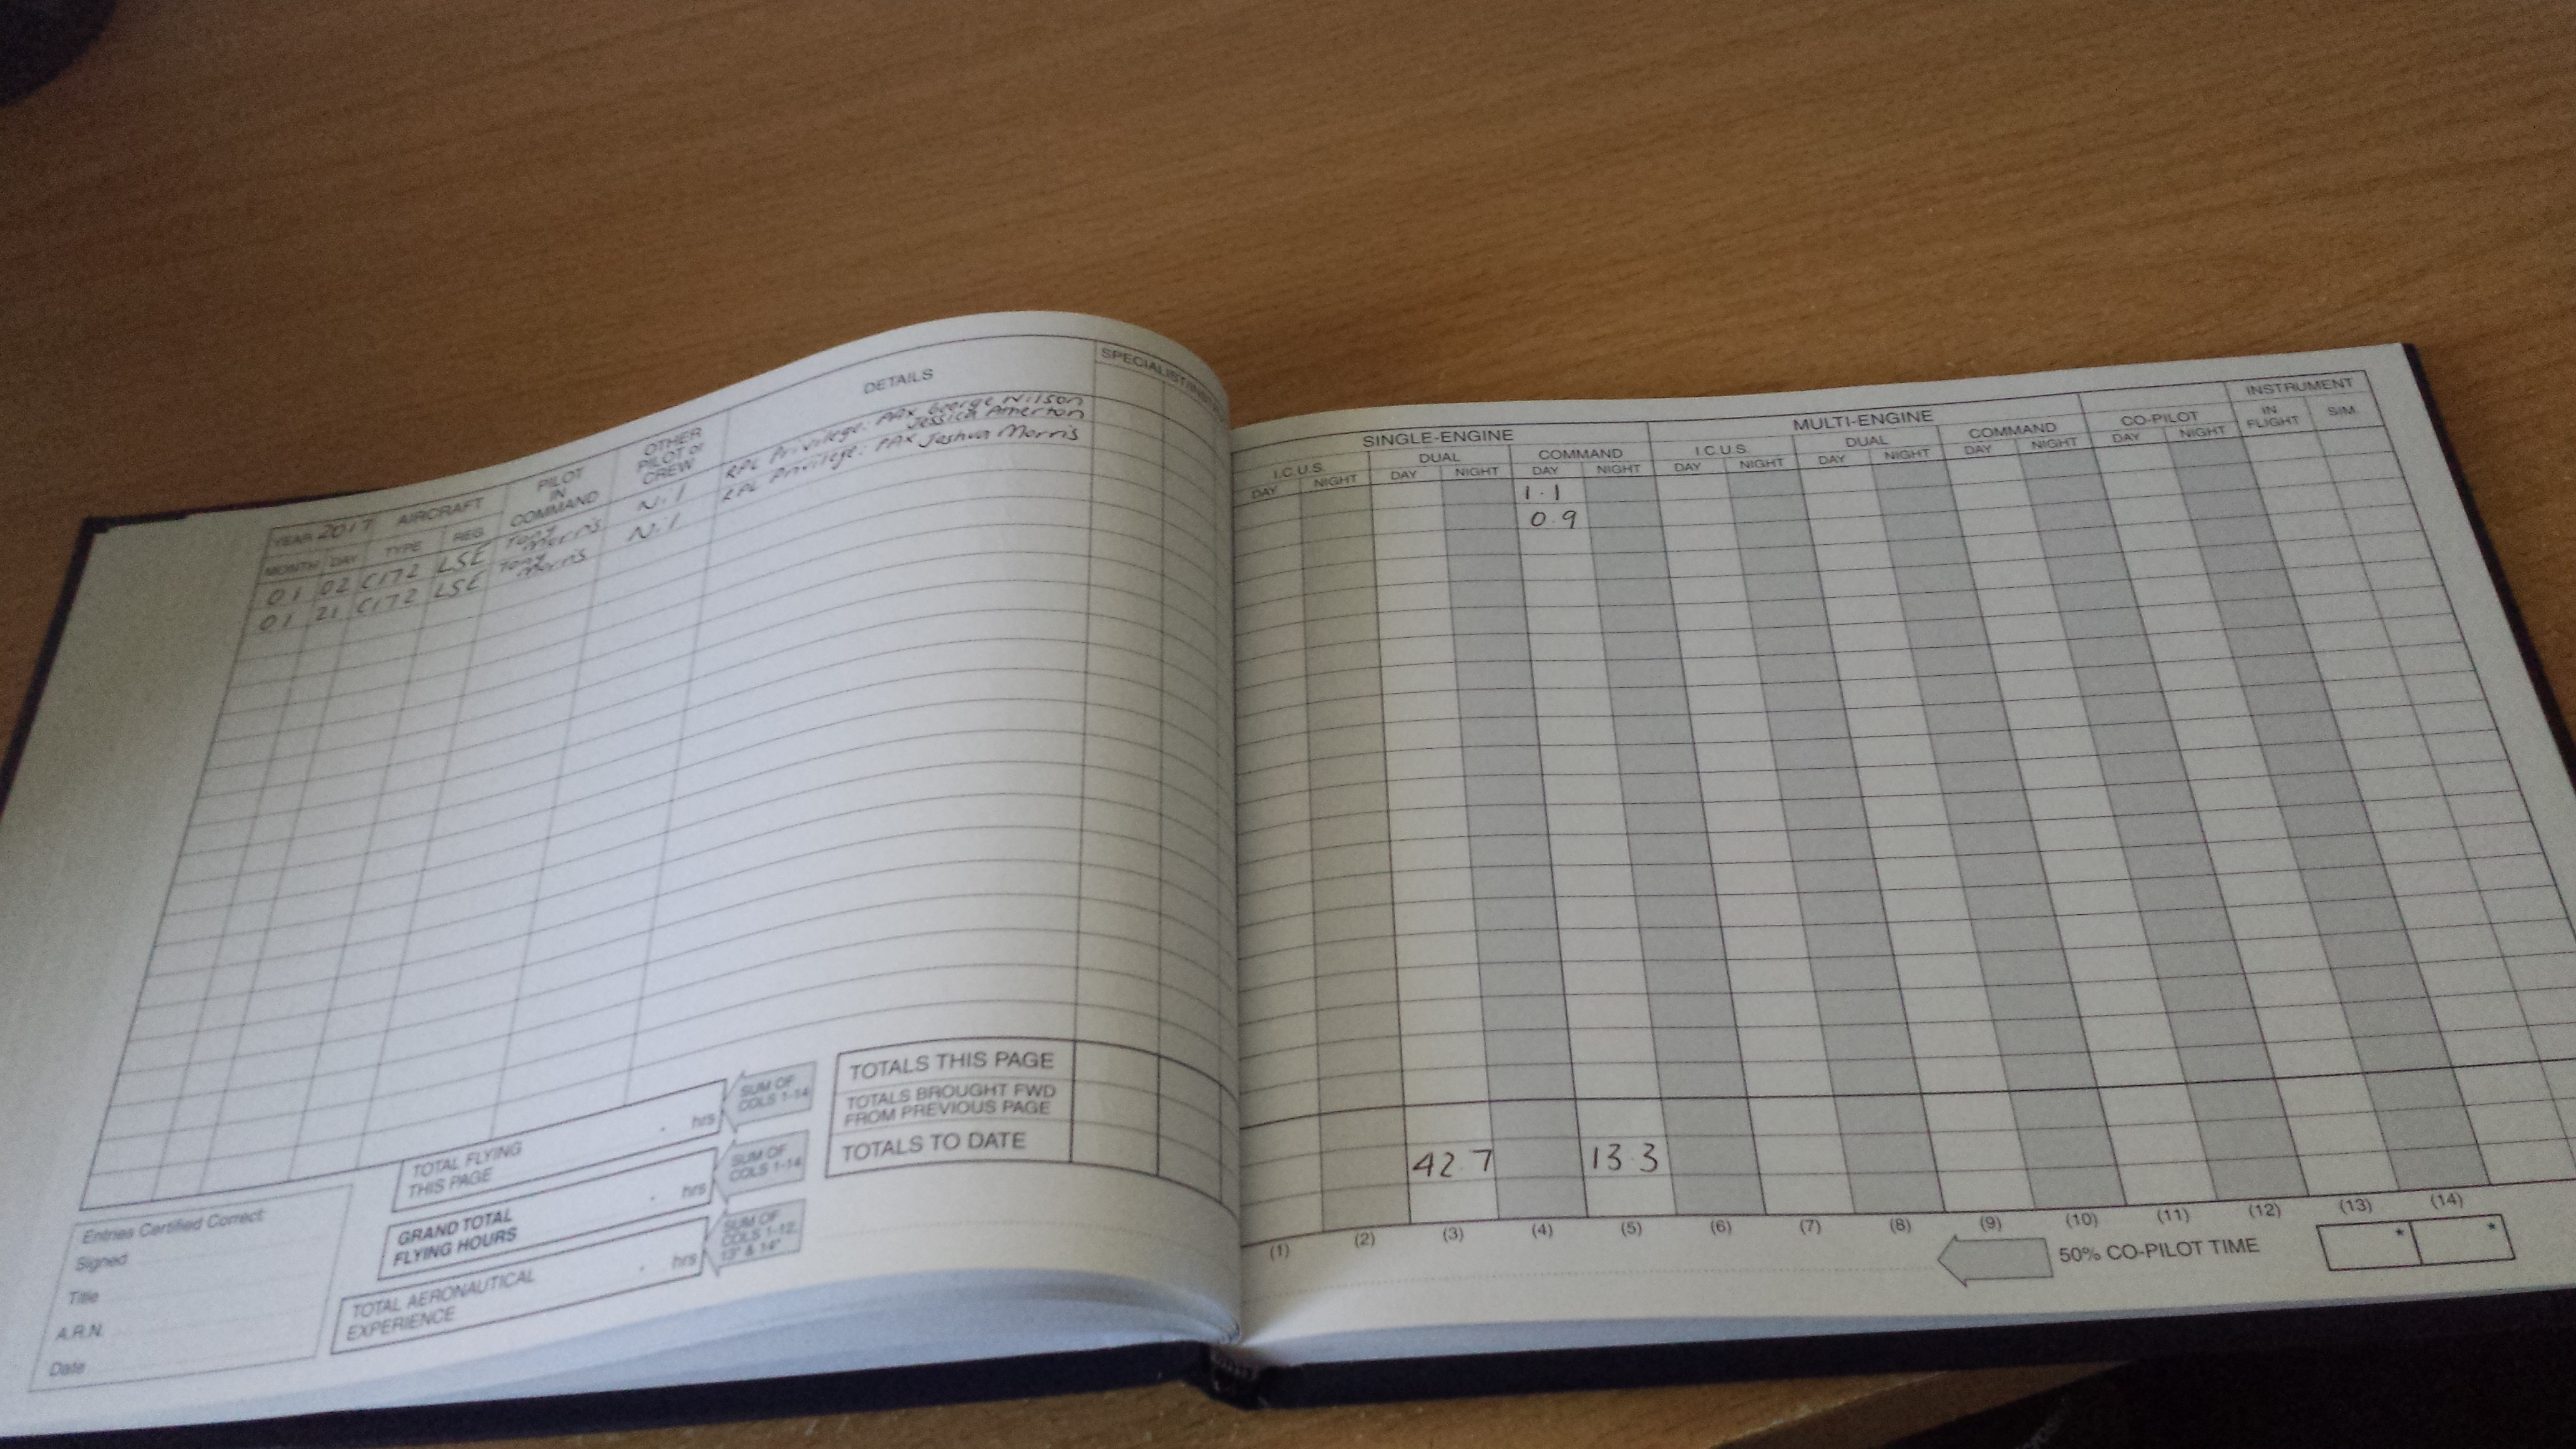
\includegraphics[height=0.5\textheight]{image/logbook.jpg}
\end{block}
\end{frame}

\begin{frame}
\frametitle{Pilot Logbooks}
\begin{block}{CASR1998 REG 61.345 \emph{(pilot logbooks)}}
Are electronic logbooks OK?
\end{block}
\end{frame}

\begin{frame}
\frametitle{Pilot Logbooks}
\begin{block}{Yes. CASR1998 REG 61.365(3)}
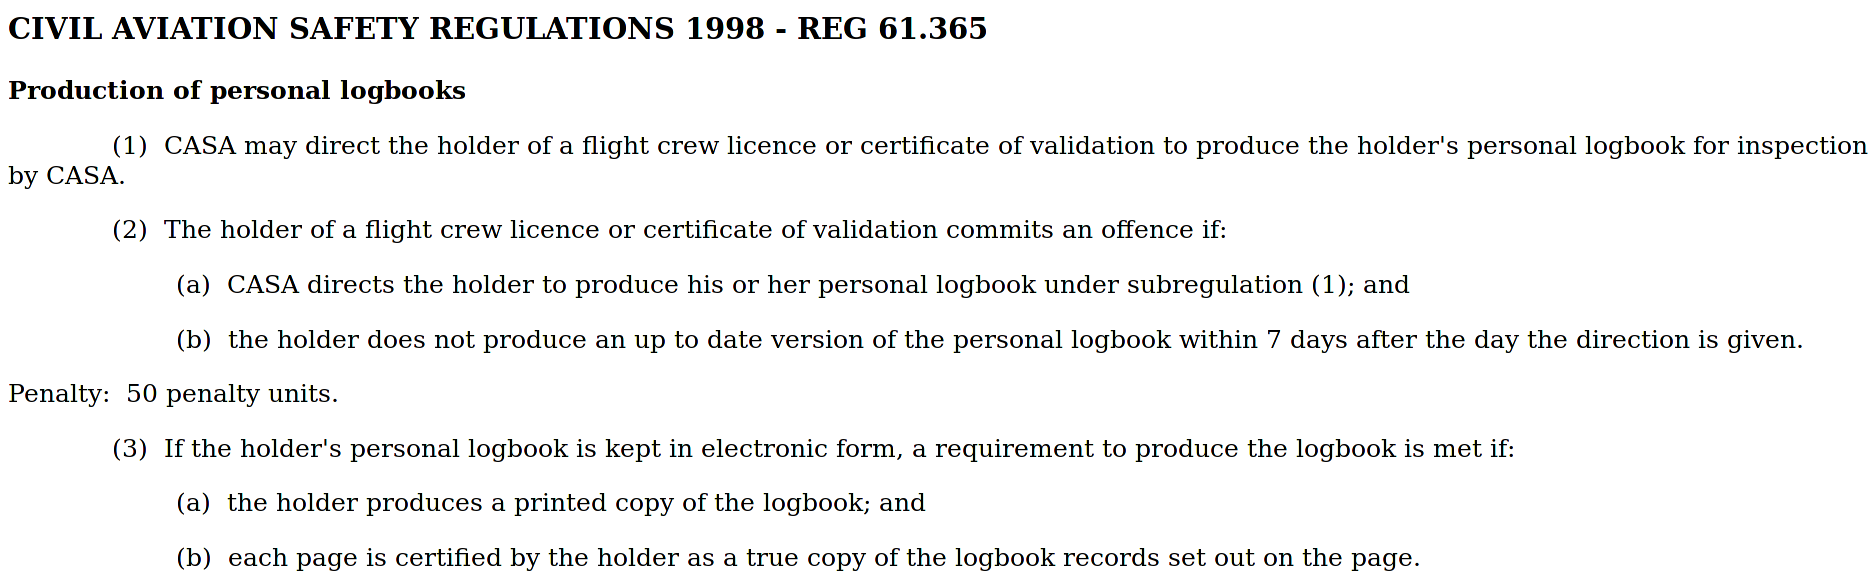
\includegraphics[height=0.3\textheight]{image/casr-logbook-production.png}
\end{block}
\end{frame}

\begin{frame}
\frametitle{Pilot logbooks}
\begin{center}
Introducing the pilot logbook cottage industry
\par

\includegraphics[height=0.1\textheight]{image/reddit-logbooks.png}
\end{center}
\end{frame}

\begin{frame}
\frametitle{Introducing the pilot logbook cottage industry}
\begin{block}{Excel?}
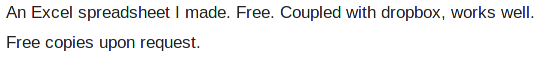
\includegraphics[height=0.1\textheight]{image/logbook-1.png}
\end{block}
\end{frame}

\begin{frame}
\frametitle{Introducing the pilot logbook cottage industry}
\begin{block}{Google spreadsheet?}
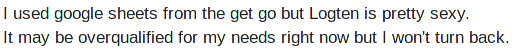
\includegraphics[height=0.1\textheight]{image/logbook-2.png}
\end{block}
\end{frame}

\begin{frame}
\frametitle{Introducing the pilot logbook cottage industry}
\begin{block}{blah blah I am hostage to proprietary crap blah blah}
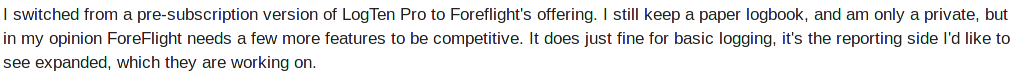
\includegraphics[height=0.08\textheight]{image/logbook-3.png}
\end{block}
\end{frame}

\begin{frame}
\frametitle{Introducing the pilot logbook cottage industry}
\begin{block}{I love proprietary crap!}
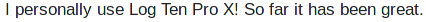
\includegraphics[height=0.05\textheight]{image/logbook-4.png}
\end{block}
\end{frame}

\begin{frame}
\frametitle{Introducing the pilot logbook cottage industry}
\begin{block}{I hate proprietary crap when it doesn't work}
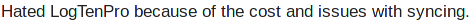
\includegraphics[height=0.05\textheight]{image/logbook-5.png}
\end{block}
\end{frame}

\begin{frame}
\begin{block}{I hate some proprietary crap, when I cross the date line}
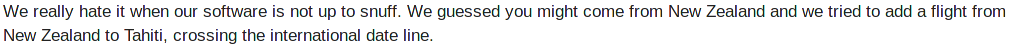
\includegraphics[height=0.05\textheight]{image/logbook-6.png}
\end{block}
\end{frame}

\begin{frame}
\frametitle{Pilot logbooks}
\begin{block}{umm where's my logbook gone?}
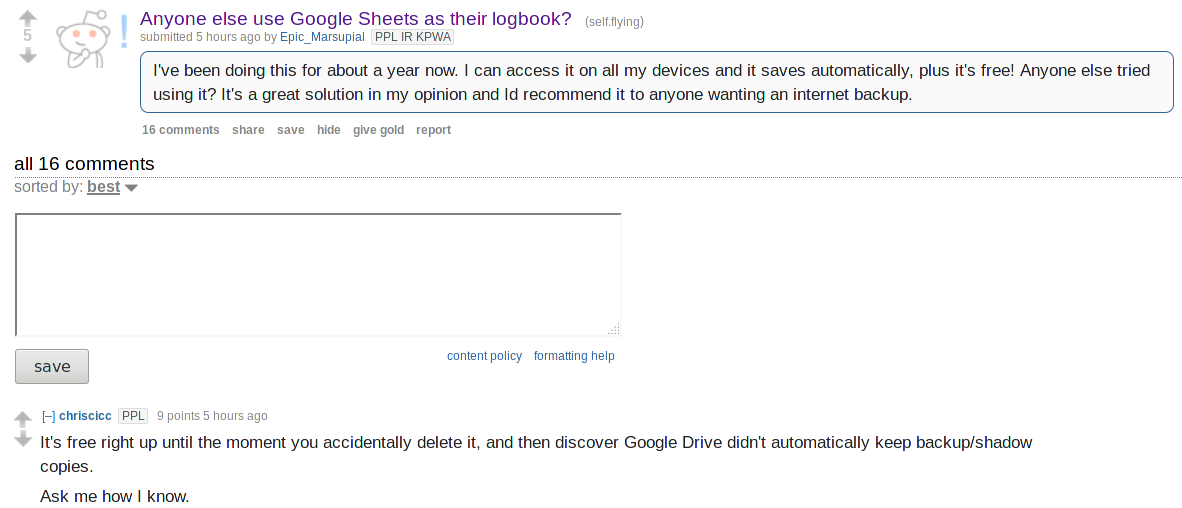
\includegraphics[height=0.4\textheight]{image/logbook-7.png}
\end{block}
\par
\tiny{\emph{01 August 2016}}
\end{frame}

\begin{frame}
\frametitle{Pilot logbooks}
\begin{block}{I put these questions out to the world}
\begin{itemize}
\item<1-> Does the accuracy of a logbook affect safety? Efficiency?
\item<2-> Does the ability to query a logbook affect accuracy?
\item<3-> Does the reliability of a logbook affect safety?
\item<4-> \textbf{Should a logbook be subject to the same data management standards we programmers apply to our source code?}
\end{itemize}

\end{block}
\end{frame}

\begin{frame}
\frametitle{Pilot logbooks}
\begin{block}{Pilot logbook requirements}
\begin{itemize}
\item<1-> Data loss impossible, including logbook history, with merge.
\item<2-> First-class logbook-related data type values for composition.
\item<3-> Values that can \emph{close over} other values (function arguments).
\item<4-> Ability for \emph{arbitrary} reporting.
\item<5-> \textbf{You can see where I am going, innit?}
\end{itemize}
\end{block}
\end{frame}

\begin{frame}
\frametitle{Pilot logbook}
\begin{block}{A responsible, CASR1998 REG 61.x compliant pilot uses}
\begin{itemize}
\item<1-> Haskell data type (sums and products) for logbook.
\item<1-> Lenses for querying and reporting.
\item<1-> Pilot logbook zipper for navigating a logbook.
\item<1-> A pretty-printer to meet CASR1998 REG 61.365 requirements.
\item<1-> Revision control (git) for maintaining zero data loss.
\item<1-> Publishes open-source logbook libraries as a good citizen.
\end{itemize}
\end{block}
\end{frame}

\begin{frame}[fragile]
\frametitle{Use-case}
\begin{block}{Query: Aviation Reference Number (ARN) of logbook owner}
\begin{lstlisting}[style=haskell,basicstyle=\scriptsize\ttfamily,mathescape]
digitlist :: Prism$'$ Int [Digit]
arn :: Lens$'$ Aviator [Digit]
logbookaviator :: Lens$'$ Logbook Aviator
mylogbook :: Logbook

$\lambda$> mylogbook ^.
      logbook . logbookaviator . arn . re digitlist
1007036
\end{lstlisting}
\end{block}
\end{frame}

\begin{frame}[fragile]
\frametitle{Use-case}
\begin{block}{Modify: Set the digit at index 2 of the ARN to 5}
\begin{lstlisting}[style=haskell,basicstyle=\scriptsize\ttfamily,mathescape]
arn :: Lens$'$ Aviator [Digit]
logbookaviator :: Lens$'$ Logbook Aviator

$\lambda$> :t logbook . logbookaviator . arn %~
      \d -> d & ix 2 .~ x5
Logbook -> Logbook
\end{lstlisting}
\end{block}
\end{frame}

\begin{frame}[fragile]
\frametitle{Use-case}
\begin{block}{Modify: Upper-case the surname of the logbook owner}
\begin{lstlisting}[style=haskell,basicstyle=\scriptsize\ttfamily,mathescape]
logbookaviator :: Lens$'$ Logbook Aviator
surname :: Lens$'$ Aviator String
map toUpper :: String -> String

$\lambda$> :t over
      (logbook . logbookaviator . surname)
      (map toUpper)
Logbook -> Logbook
\end{lstlisting}
\end{block}
\end{frame}

\begin{frame}[fragile]
\frametitle{Use-case}
\begin{block}{Query: Aircraft from all flights}
\begin{lstlisting}[style=haskell,basicstyle=\scriptsize\ttfamily,mathescape]
logbookentries :: Lens Logbook Entries
_Wrapped :: Iso$'$ Entries [Entry]
folded :: Foldable f => IndexedFold Int (f a) a 
_AircraftFlightEntry ::
      Prism$'$ Entry AircraftFlight
flightaircraft :: Lens$'$ AircraftFlight Aircraft
mylogbook :: Logbook

$\lambda$> :t mylogbook ^..
      logbook .
      logbookentries .
      _Wrapped .
      folded .
      _AircraftFlightEntry .
      flightaircraft
[Aircraft]
\end{lstlisting}
\end{block}
\end{frame}

\begin{frame}[fragile]
\frametitle{Use-case}
\begin{block}{Query: Find first flight in aircraft registration VH-VVO}
\begin{lstlisting}[style=haskell,basicstyle=\scriptsize\ttfamily,mathescape]
logbookentries :: Lens Logbook Entries
_AircraftFlightEntry ::
      Prism$'$ Entry AircraftFlight
flightaircraft :: Lens$'$ AircraftFlight Aircraft
aircraftRegistration :: Lens$'$ Aircraft String

$\lambda$> :t findOf
      ( logbook . 
        logbookentries . 
        _Wrapped . 
        folded . 
        _AircraftFlightEntry)
        ( elemOf
          (
            flightaircraft . 
            aircraftRegistration)
          "VH-VVO")
      mylogbook
Maybe AircraftFlight
\end{lstlisting}
\end{block}
\end{frame}

\begin{frame}[fragile]
\frametitle{Use-case}
\begin{block}{Print: pretty-print all exam results}
\begin{lstlisting}[style=haskell,basicstyle=\scriptsize\ttfamily,mathescape]
_ExamEntry ::
      Prism$'$ Entry Exam
examResult :: Lens$'$ Exam Int
examResultMaximum :: Lens$'$ Exam Int

$\lambda$> mapMOf_
      ( logbook . logbookentries .
        _Wrapped . folded .
        _ExamEntry .
        runGetter
          ((\x y -> show x ++ $\text{" out of "}$ ++ show y) <$\text{\$}$>
          Getter examResult <*>
          Getter examResultMaximum)
        )
      putStrLn
      mylogbook
31 out of 40
38 out of 40
38 out of 40
\end{lstlisting}
\end{block}
\end{frame}

\begin{frame}[fragile]
\frametitle{Use-case}
\begin{block}{Query: All aircraft flights as pilot in-command}
\begin{lstlisting}[style=haskell,basicstyle=\scriptsize\ttfamily,mathescape]
logbookentries :: Lens Logbook Entries
_AircraftFlightEntry ::
      Prism$'$ Entry AircraftFlight
flightaircraft :: Lens$'$ AircraftFlight Aircraft
aircraftRegistration :: Lens$'$ Aircraft String

$\lambda$> :t
      mylogbook ^..
      logbook .
      logbookentries .
      _Wrapped .
      folded .
      _AircraftFlightEntry .
      filtered
        (elemOf (command . _InCommand) ())
[AircraftFlight]
\end{lstlisting}
\end{block}
\end{frame}

\begin{frame}[fragile]
\frametitle{Use-case}
\begin{block}{Query: Total day hours as pilot in-command}
\begin{lstlisting}[style=haskell,basicstyle=\scriptsize\ttfamily,mathescape]
$\lambda$> foldOf
      ( logbook .
        logbookentries .
        _Wrapped .
        folded .
        _AircraftFlightEntry .
        filtered
          (elemOf (command . _InCommand) ()) .
        daynight .
        dayDayNight
      )
      mylogbook
TimeAmount {_hours = 4, _tenthofhour = 8}
\end{lstlisting}
\end{block}
\end{frame}

\begin{frame}[fragile]
\frametitle{Use-case}
\begin{block}{Print the entire logbook to a single, printable HTML web page \emph{CASR1998 REG 61.365}}
\begin{lstlisting}[style=haskell,mathescape]
$\lambda$> :t htmlLogbook mylogbook
Html ()
\end{lstlisting}
\end{block}
\href{http://logbook.aviation.tmorris.net/}{http://logbook.aviation.tmorris.net/}
\end{frame}

\begin{frame}[fragile]
\frametitle{Use-case}
\begin{block}{Query of arbitrary obtuseness}
All flights where, if the departure and arrival date is the same day (UTC), and that date-of-month is a multiple of 7, unless either there was an intermediate flight path point of YSCN, or the time the logbook owner was PiC for the first three legs of the flight, is between 2.0 hours and the total sum of hours of dual flight in aircraft registered VH-AFR.
\end{block}
\end{frame}

\begin{frame}[fragile]
\frametitle{Use-case}
\begin{block}{End goal}
\begin{itemize}
\item<1-> The effort required to perform a query or update is directly proportional to the sophistication of that request.
\item<2->\sout{``no the software does not \textbf{let you} do that.''}
\item<3-> Software is my slave, not the other way around.
\end{itemize}
\end{block}
\end{frame}
